\documentclass{beamer}
\usetheme{Berlin}
\usecolortheme[light,accent=blue]{solarized}
\usepackage{fontspec}
\usepackage{xunicode}
\usepackage{xltxtra}
\setmainfont{DejaVuSans}
\usepackage{booktabs}
\usepackage{lmodern}
\usepackage{listings}
\usepackage{color}
\usepackage{tikz}
\usetikzlibrary{trees, shapes.misc, arrows}
\usepackage{fancyvrb}
\usepackage{pgfkeys}
\usepackage{graphicx}
\usepackage[normalem]{ulem}
\graphicspath{{./images/}}
\setbeamertemplate{headline}{}

\lstset{%
    basicstyle=\footnotesize{}\ttfamily{},
    breakatwhitespace=false,
    breaklines=true,
    captionpos=b,
    frame=signle,
    keepspaces=true,
    columns=flexible,
    language=bash,
    numbers=none,
    numbersep=5pt,
    numberstyle=\tiny\color{solarizedBase00},
    showspaces=false,
    showstringspaces=false,
    stepnumber=1,
    showtabs=false,
    tabsize=2
}

\title{Learning Git± in Reverse}
\subtitle{A Backwards Introduction to \\{} the ``information manager from
hell'' [e83c51633]}
\author[Ballou]{Kenny Ballou}
\institute[/dev/null]{/dev/null > labs}

\AtBeginSection[]{%
    \begin{frame}
    \tableofcontents[
        currentsection,
        sectionstyle=show/shaded,
        subsectionstyle=show/show/hide]
    \end{frame}
}

\begin{document}
% TikZ Styles
\tikzstyle{every node}=[%
    fill=solarizedBase02,
    draw=solarizedBase01,
    thick,
    rounded corners,
    anchor=north,
    sibling distance=6cm]
\tikzstyle{edge from parent}=[%
    solarizedBase00,
    -o,
    thick,
    draw]

%\tikzstyle{edge from parent path}=[%
%    \tikzparentnode.east |- \tikzchildnode.south]

\begin{frame}[label=titleslide]
\titlepage{}
\end{frame}

\begin{frame}
\tableofcontents[subsectionstyle=hide]
\end{frame}

\begin{frame}
\frametitle{About Me}
\begin{itemize}
\item{Hacker}
\item{Developer (read gardener)}
\item{Mathematician}
\item{Student}
\item{\href{https://twitter.com/kennyballou}{@kennyballou}}
\item{\href{https://github.com}{github/kennyballou}}
\item{\url{https://git.devnulllabs.io}}
\item{\url{https://kennyballou.com}}
\end{itemize}

\end{frame}

\begin{frame}
  \frametitle{About You}
  \begin{itemize}
  \item<2->{Heard of Git± before}
  \item<3->{Used Git± before}
  \item<4->{Use Git± daily}
  \item<5->{Have attended this talk before}
  \item<6->{Consider yourself a Git± master}
  \end{itemize}
\end{frame}

\section{Introduction}

\begin{frame}
\begin{figure}

\includegraphics[scale=0.45]{xkcd_git.png}
\caption{XKCD on Git\cite{website:xkcd_git_comic}}
\end{figure}
\end{frame}

\subsection{Information Manager from Hell}
\begin{frame}
\frametitle{Git±}
\framesubtitle{What is Git?}
\begin{itemize}
\item<2->{Distributed Version Control System (D-VCS)}
\item<3->{``A way to manage code''}
\item<4->{``My preferred VCS tool''}
\item<5->{The ``information manager from hell''}
\item<6->{A distributed DAG}
\begin{itemize}
\item<6->{``A Graph Tree''}
\end{itemize}
\item<7->{An object store}
\item<8->{A content addressable filesystem}
\item<9->{A key-value store}
\end{itemize}
\end{frame}

\begin{frame}
\frametitle{Git±}
What does Git store?
\begin{itemize}
\item<2-6>{Objects}
\item<3-5>{Commits}
\item<4-5>{Code}
\item<5-5>{``Packs''}
\end{itemize}
\end{frame}

\subsection{Terms and Definitions}
\begin{frame}
\frametitle{Git Definitions}
\begin{itemize}
\item{Objects}
\item{Trees}
\item{Commits}
\end{itemize}
\end{frame}

\begin{frame}
\frametitle{Git Definitions}
\framesubtitle{``It's turtles all the down''}
\begin{itemize}
\item{Objects}
\item{Trees ← object}
\item{Commits ← object}
\end{itemize}
\end{frame}

\section{Git± Plumbing}

\begin{frame}[fragile]
\frametitle{Initializing a Repository the Hard Way}
\lstinputlisting{code/1/1}
\end{frame}

\begin{frame}[fragile]
\frametitle{Initialization Results}
\lstinputlisting{code/1/2}
\end{frame}

\subsection{Blobs}
\begin{frame}
\frametitle{Git Objects}
\begin{itemize}
\item{ZLIB compressed blob}
\item{Dumb containers, storing provided content}
\item{Created using the \texttt{git-hash-object} plumbing command}
\end{itemize}
\end{frame}

\begin{frame}[fragile]
\frametitle{\texttt{git-hash-object}}
\lstinputlisting{code/1/3}
\end{frame}

\begin{frame}[fragile]
\frametitle{\texttt{git-hash-object}}
\lstinputlisting{code/1/4}
\end{frame}

\begin{frame}
\frametitle{Git Objects}
\begin{figure}
\begin{tikzpicture}
    \node[text=solarizedBlue] at (0,  0) {257cc5642}
        child{node[text=solarizedGreen] {foo}};
    \node[text=solarizedBlue] at (3,  0) {5716ca598}
        child{node[text=solarizedGreen] {bar}};
\end{tikzpicture}
\end{figure}
\end{frame}


\begin{frame}[fragile]
\frametitle{\texttt{git-cat-file}}
\lstinputlisting{code/1/5}
\end{frame}

\begin{frame}[fragile]
\frametitle{Raw Access to Git Objects}
\lstinputlisting{code/1/6}
\end{frame}

\begin{frame}
\frametitle{Git Object Limitations}
\begin{itemize}
\item{Remembering 40 character SHA's is hard}
\item{What about file names?}
\end{itemize}
\end{frame}

\subsection{Trees}

\begin{frame}
\frametitle{Git Trees}
\begin{itemize}
\item{ZLIB compressed blobs}
\item{Contain references to files and other trees}
\item{Created using the \texttt{git-update-index} and \texttt{git-write-tree}}
\end{itemize}
\end{frame}

\begin{frame}[fragile]
\frametitle{\texttt{git-update-index} and \texttt{git-write-tree}}
\lstinputlisting{code/2/1}
\end{frame}

\begin{frame}
\frametitle{Git± Tree File Modes}
\begin{description}
\item[100644]{Regular file, *nix permissions 0644}
\item[100755]{Regular file, *nix permissions 0755, e.g., executable}
\item[120000]{Symbolic link}
\item[160000]{``Gitlink'', object from another repository, \texttt{fast-import}}
\item[040000]{Subdirectory, \texttt{fast-import}}
\end{description}
\end{frame}

\begin{frame}[fragile]
\frametitle{Current Git Objects}
\lstinputlisting{code/2/2}
\end{frame}

\begin{frame}
\frametitle{Current Git Objects}
\begin{figure}
\begin{tikzpicture}[sibling distance=3cm]
    \node[text=solarizedMagenta] at (0, 0) {fcf0be4d7}
        child{node[text=solarizedBlue] {257cc5642}
            child{node[text=solarizedGreen]{foo}}};
    \node[text=solarizedBlue] at (3, -1) {5716ca598}
        child{node[text=solarizedGreen]{bar}};
\end{tikzpicture}
\end{figure}
\end{frame}

\begin{frame}[fragile]
\frametitle{Adding \texttt{bar.txt}}
\lstinputlisting{code/2/3}
\end{frame}

\begin{frame}[fragile]
\frametitle{Git Objects}
\lstinputlisting{code/2/4}
\end{frame}

\begin{frame}
\frametitle{Git Objects, Updated}
\begin{figure}
\begin{tikzpicture}[sibling distance=3cm]
    \node[text=solarizedMagenta] at (0, 0) {b98c9a9f}
        child{node[text=solarizedBlue] (foo_hash) {257cc5642}
            child{node[text=solarizedGreen]{foo}}}
        child{node[text=solarizedBlue] {5716ca598}
            child{node[text=solarizedGreen] {bar}}};
    \node[text=solarizedMagenta] at (-3, 0) (previous_hash) {fcf0be4d7};
    \node at (-3, 1.5) (previous) {Previous Tree};
    \draw[-o,thick] (previous_hash) -- (foo_hash);
    \draw[->,thick] (previous) -- (previous_hash);
\end{tikzpicture}
\end{figure}
\end{frame}

\begin{frame}[fragile]
\frametitle{Modifying Files}
\lstinputlisting{code/2/5}
\end{frame}

\begin{frame}
\frametitle{Git Objects, Updated}
\begin{figure}
\begin{tikzpicture}[sibling distance=3cm]
    \node[text=solarizedMagenta] at (4, 0) {68b75754}
        child{node[text=solarizedBlue] (bar_hash) {5716ca598}
            child{node[text=solarizedGreen] {bar}}}
        child{node[text=solarizedBlue] {a3f555b64}
            child{node[text=solarizedGreen]{foo 2}}};
    \node[text=solarizedMagenta] at (0, 0) (previous_hash) {b98c9a9f}
        child{node[text=solarizedBlue] (foo_hash) {257cc5642}
            child{node[text=solarizedGreen]{foo}}};
    \node at (0, 1.5) (previous) {Previous Tree};
    \draw[-o,thick] (previous_hash) -- (bar_hash);
    \draw[->,thick] (previous) -- (previous_hash);
\end{tikzpicture}
\end{figure}
\end{frame}

\begin{frame}[fragile]
\frametitle{Modifying Files}
\framesubtitle{Current Objects}
\lstinputlisting{code/2/6}
\end{frame}

\begin{frame}
\frametitle{Modifying Files}
\framesubtitle{Current Objects}
\begin{figure}
\begin{tikzpicture}[sibling distance=3cm]
    \node at (0, 0) {Old Tree}
        child{node[text=solarizedMagenta] {b98c9a9f}
        child{node[text=solarizedBlue] {257cc5642}
            child{node[text=solarizedGreen]{foo}}}
        child{node[text=solarizedBlue] {5716ca598}
            child{node[text=solarizedGreen] {bar}}}};
    \node at (5, 0) {Current Tree}
        child{node[text=solarizedMagenta] {68b75754}
            child{node[text=solarizedBlue] {5716ca598}
                child{node[text=solarizedGreen] {bar}}}
            child{node[text=solarizedBlue] {a3f555b64}
                child{node[text=solarizedGreen]{foo 2}}}};
\end{tikzpicture}
\end{figure}
\end{frame}

\begin{frame}
\frametitle{Current Objects}
\framesubtitle{The Beginnings of a DAG}
\begin{figure}
\begin{tikzpicture}[sibling distance=3cm]
    \node at (0, 0) {Old Tree}
        child{node[text=solarizedMagenta] {b98c9a9f}
        child{node[text=solarizedBlue] {257cc5642}
            child{node[text=solarizedGreen]{foo}}}
        child{node[text=solarizedBlue] (bar_hash) {5716ca598}
            child{node[text=solarizedGreen] {bar}}}};
    \node at (4, 0) {Current Tree}
        child{node[text=solarizedMagenta] (new_tree) {68b75754}
            child{node[text=solarizedBlue] {a3f555b64}
                child{node[text=solarizedGreen]{foo 2}}}};
    \draw[-o,thick] (new_tree) edge (bar_hash);
\end{tikzpicture}
\end{figure}
\end{frame}

\begin{frame}
\frametitle{Limitation of Git± Trees}
\begin{itemize}
\item{Remembering SHA's is \textit{still} hard}
\item{No metadata about who, when, and why}
\end{itemize}
\end{frame}

\subsection{Commits}

\begin{frame}
\frametitle{Git± Commit Objects}
\begin{itemize}
\item{ZLIB compressed blob}
\item{Stores metadata about changes}
\item{Stores a reference to the tree being saved}
\item{Created using \texttt{git-commit-tree}}
\end{itemize}
\end{frame}

\begin{frame}[fragile]
\frametitle{\texttt{git-commit-tree}}
\lstinputlisting{code/3/1}
\end{frame}

\begin{frame}
\frametitle{\texttt{git-commit-tree}}
\begin{figure}
\begin{tikzpicture}
    \node[text=solarizedCyan] {0e7ce0c}
        child{node[text=solarizedMagenta] {fcf0be4d7}
            child{node[text=solarizedBlue] {257cc5642}
                child{node[text=solarizedGreen]{foo}}}};
\end{tikzpicture}
\end{figure}
\end{frame}

\begin{frame}[fragile]
\frametitle{\texttt{git-commit-tree}}
\lstinputlisting{code/3/2}
\end{frame}

\begin{frame}
\frametitle{\texttt{git-commit-tree}}
\begin{figure}
\begin{tikzpicture}[sibling distance=3cm]
    \node[text=solarizedCyan] {69ea0e9}
        child{node[text=solarizedCyan] {0e7ce0c}}
        child{node[text=solarizedMagenta] {b98c9a9f9}
            child{node[text=solarizedBlue] {5716ca598}
                child{node[text=solarizedGreen] {bar}}}
            child{node[text=solarizedBlue] {257cc5642}
                child{node[text=solarizedGreen]{foo}}}};
\end{tikzpicture}
\end{figure}
\end{frame}

\begin{frame}[fragile]
\frametitle{\texttt{git-commit-tree}}
\lstinputlisting{code/3/3}
\end{frame}

\begin{frame}
\frametitle{\texttt{git-commit-tree}}
\begin{figure}
\begin{tikzpicture}[sibling distance=3cm]
    \node[text=solarizedCyan] {32a5f01}
        child{node[text=solarizedCyan] {69ea0e9}}
        child{node[text=solarizedMagenta] {68b757546}
            child{node[text=solarizedBlue] {5716ca598}
                child{node[text=solarizedGreen] {bar}}}
            child{node[text=solarizedBlue] {a3f555b64}
                child{node[text=solarizedGreen]{foo 2}}}};
\end{tikzpicture}
\end{figure}
\end{frame}

\begin{frame}[fragile]
\frametitle{Git± History}
\lstinputlisting{code/3/4}
\end{frame}

\begin{frame}
\frametitle{Git± Thus Far}
\begin{figure}
\begin{tikzpicture}
    \node[text=solarizedBlue] (foo) at (10, -10) {foo};
\end{tikzpicture}
\end{figure}
\end{frame}

\begin{frame}
\frametitle{Git± Thus Far}
\begin{figure}
\begin{tikzpicture}
    \node[text=solarizedBlue] (foo) at (10, -10) {foo};
    \node[text=solarizedBlue] (hfoo) at (10, -8) {257cc564};
    \draw[-o,thick] (hfoo) -- (foo);
\end{tikzpicture}
\end{figure}
\end{frame}

\begin{frame}
\frametitle{Git± Thus Far}
\begin{figure}
\begin{tikzpicture}
    \node[text=solarizedBlue] (foo) at (10, -10) {foo};
    \node[text=solarizedBlue] (hfoo) at (10, -8) {257cc564};
    \node[text=solarizedMagenta] (tree1) at (9, -6) {fcf0be4d};
    \draw[-o,thick] (hfoo) -- (foo);
    \draw[-o,thick] (tree1) -- (hfoo);
\end{tikzpicture}
\end{figure}
\end{frame}

\begin{frame}
\frametitle{Git± Thus Far}
\begin{figure}
\begin{tikzpicture}
    \node[text=solarizedBlue] (foo) at (10, -10) {foo};
    \node[text=solarizedBlue] (hfoo) at (10, -8) {257cc564};
    \node[text=solarizedMagenta] (tree1) at (9, -6) {fcf0be4d};
    \node[text=solarizedCyan] (commit1) at (5, -6) {0e7ce0c};
    \draw[-o,thick] (hfoo) -- (foo);
    \draw[-o,thick] (tree1) -- (hfoo);
    \draw[-o,thick] (commit1) -- (tree1);
\end{tikzpicture}
\end{figure}
\end{frame}

\begin{frame}
\frametitle{Git± Thus Far}
\begin{figure}
\begin{tikzpicture}
    \node[dashed,text=solarizedBlue] (foo) at (10, -10) {foo};
    \node[text=solarizedBlue] (bar) at (8,  -10) {bar};
    \node[dashed,text=solarizedBlue] (hfoo) at (10, -8) {257cc564};
    \node[text=solarizedBlue] (hbar) at (8,  -8) {5716ca59};
    \node[text=solarizedMagenta] (tree1) at (9, -6) {fcf0be4d};
    \node[text=solarizedCyan] (commit1) at (5, -6) {0e7ce0c};
    \draw[-o,thick] (hfoo) -- (foo);
    \draw[-o,thick] (hbar) -- (bar);
    \draw[-o,thick] (tree1) -- (hfoo);
    \draw[-o,thick] (commit1) -- (tree1);
\end{tikzpicture}
\end{figure}
\end{frame}

\begin{frame}
\frametitle{Git± Thus Far}
\begin{figure}
\begin{tikzpicture}
    \node[dashed,text=solarizedBlue] (foo) at (10, -10) {foo};
    \node[text=solarizedBlue] (bar) at (8,  -10) {bar};
    \node[dashed,text=solarizedBlue] (hfoo) at (10, -8) {257cc564};
    \node[text=solarizedBlue] (hbar) at (8,  -8) {5716ca59};
    \node[text=solarizedMagenta] (tree2) at (9, -6) {b98c9a9f9};
    \node[text=solarizedCyan] (commit2) at (5, -6) {69ea0e9};
    \node[text=solarizedCyan] (commit1) at (5, -8) {0e7ce0c};
    \draw[-o,thick] (hfoo) -- (foo);
    \draw[-o,thick] (hbar) -- (bar);
    \draw[-o,thick] (tree2) -- (hfoo);
    \draw[-o,thick] (tree2) -- (hbar);
    \draw[-o,thick] (commit2) -- (tree2);
    \draw[-o,thick] (commit2) -- (commit1);
\end{tikzpicture}
\end{figure}
\end{frame}

\begin{frame}
\frametitle{Git± Thus Far}
\begin{figure}
\begin{tikzpicture}
    \node[text=solarizedBlue] (foo) at (10, -10) {foo 2};
    \node[dashed,text=solarizedBlue] (bar) at (8,  -10) {bar};
    \node[text=solarizedBlue] (hfoo) at (10, -8) {a3f555b6};
    \node[dashed,text=solarizedBlue] (hbar) at (8,  -8) {5716ca59};
    \node[text=solarizedMagenta] (tree3) at (9, -6) {68b75754};
    \node[text=solarizedCyan] (commit3) at (5, -6) {32a5f01};
    \node[text=solarizedCyan] (commit2) at (5, -8) {69ea0e9};
    \node[text=solarizedCyan] (commit1) at (5, -10) {0e7ce0c};
    \draw[-o,thick] (hfoo) -- (foo);
    \draw[-o,thick] (hbar) -- (bar);
    \draw[-o,thick] (tree2) -- (hfoo);
    \draw[-o,thick] (tree2) -- (hbar);
    \draw[-o,thick] (commit3) -- (tree3);
    \draw[-o,thick] (commit3) -- (commit2);
    \draw[-o,thick] (commit2) -- (commit1);
\end{tikzpicture}
\end{figure}
\end{frame}

\subsection{Packfiles}

\begin{frame}
\frametitle{Git± Packfiles}
\begin{itemize}
\item<2->{Tight Object Storage}
\item<3->{``Packs'' Objects Together}
\item<4->{Adds quick, indexed access to objects}
\item<5->{Motivated for network and access efficiency}
\begin{itemize}
\item<5->{Not Disk Space Efficiency}
\end{itemize}
\item<6->{Created automatically}
\end{itemize}
\end{frame}

\begin{frame}
\frametitle{Creating Packfiles}
\begin{itemize}
\item<1->{\texttt{git-pack-objects}}
\item<2->{\texttt{git-gc}}
\end{itemize}
\end{frame}

\begin{frame}[fragile]
\frametitle{Creating Packfiles}
\framesubtitle{\texttt{git-pack-objects}}
\lstinputlisting[%
    basicstyle=\scriptsize{}\ttfamily{}]{code/packfiles/1}
\end{frame}

\begin{frame}[fragile]
\frametitle{Creating Packfiles}
\framesubtitle{\texttt{git-pack-objects}}
\lstinputlisting{code/packfiles/2}
\end{frame}

\begin{frame}[fragile]
\frametitle{Creating Packfiles}
\framesubtitle{\texttt{git-gc}}
\lstinputlisting{code/packfiles/3}
\end{frame}

\begin{frame}
\frametitle{Git± Packfiles}
\begin{itemize}
\item{``Tight Object Format''}
\item{Opaque Format}
\begin{itemize}
\item{Not Accessible}
\end{itemize}
\item{Plumbing commands will still work}
\end{itemize}
\end{frame}

\section{Using Git±}
\begin{frame}
\frametitle{Using Git±}
\framesubtitle{The porcelain over the pipes}
\begin{itemize}
\item{Plumbing commands are difficult, painful, and error prone}
\item{Thankfully, we have friendly ``porcelain'' commands}
\item{The basics can be covered with \texttt{git-add} and \texttt{git-commit}}
\end{itemize}
\end{frame}

\subsection{git-init}
\begin{frame}
\frametitle{\texttt{git-init}}
\begin{itemize}
\item{Create new local repository}
\item{Better than manually creating a repository}
\end{itemize}
\end{frame}

\begin{frame}[fragile]
\frametitle{\texttt{git-init}}
\lstinputlisting[basicstyle=\scriptsize{}\ttfamily{}]{code/4/git-init}
\end{frame}

\subsection{git-status}
\begin{frame}
\frametitle{\texttt{git-status}}
\begin{itemize}
\item{The go-to command for peering into the current state of a repository}
\item{Provides information about state of all files}
\begin{itemize}
\item{Currently untracked files}
\item{Currently modified files}
\item{Current state of ``staging'' area}
\end{itemize}
\end{itemize}
\end{frame}

\subsection{git-add}
\begin{frame}
\frametitle{\texttt{git-add}}
Combines:
\begin{itemize}
\item{\texttt{git-hash-object}}
\item{\texttt{git-update-index}}
\end{itemize}
\end{frame}

\begin{frame}[fragile]
\frametitle{\texttt{git-add}}
\lstinputlisting{code/4/1}
\end{frame}

\subsection{git-commit}
\begin{frame}
\frametitle{\texttt{git-commit}}
\begin{itemize}
\item{Creates a ``commit'' out of the current staging area}
\begin{itemize}
\item{Requires a short message}
\item{Will implicitly figure out the parent commit}
\item{Forwards the \texttt{HEAD} pointer and the current branch pointer}
\end{itemize}
\end{itemize}
\end{frame}

\begin{frame}[fragile]
\frametitle{\texttt{git-commit}}
\lstinputlisting{code/4/2}
\end{frame}

\subsection{git-mv}
\begin{frame}
\frametitle{\texttt{git-mv}}
\begin{itemize}
\item{Combines:}
\begin{itemize}
\item{\texttt{mv}}
\item{\texttt{git-add}}
\end{itemize}
\item{Rename detection is automatic}
\end{itemize}
\end{frame}

\begin{frame}
\frametitle{\texttt{git-mv}}
\lstinputlisting{code/4/3}
\end{frame}

\subsection{git-rm}
\begin{frame}
\frametitle{\texttt{git-rm}}
\begin{itemize}
\item{Removes the file from working tree}
\item{Stops tracking the file}
\item{Adds the removal to the staging area}
\end{itemize}
\end{frame}

\begin{frame}[fragile]
\frametitle{\texttt{git-rm}}
\lstinputlisting{code/4/4}
\end{frame}

\begin{frame}
\frametitle{\texttt{git-rm}}
\begin{itemize}
\item{Can also use regular \texttt{rm} and \texttt{git-add}}
\end{itemize}
\end{frame}

\section{Advanced Git±}
\subsection{References}
\begin{frame}
\frametitle{Git± Branches}
\begin{itemize}
\item<2->{Named reference to a commit hash}
\item<3->{Defined in text files under \texttt{./.git/refs}}
\end{itemize}
\end{frame}

\begin{frame}[fragile]
\frametitle{Git± Branches}
\lstinputlisting{code/5/1}
\end{frame}

\begin{frame}[fragile]
\frametitle{\texttt{git-branch}}
Branches can be created with a simple invocation of \texttt{git-branch}:
\lstinputlisting{code/5/2}
\end{frame}

\begin{frame}[fragile]
\frametitle{\texttt{git-checkout}}
After the branch is created, we can switch into that branch with
\texttt{git-checkout}:
\lstinputlisting{code/5/3}
\end{frame}

\begin{frame}[fragile]
\frametitle{\texttt{git-checkout -b}}
Or, we can do all in the same command:
\lstinputlisting{code/5/4}
\end{frame}

\begin{frame}[fragile]
\frametitle{Git± Branches}
Currently, all branches are pointing to the same commit:
\lstinputlisting{code/5/5}
\end{frame}

\begin{frame}[fragile]
\frametitle{Git± Branches}
\lstinputlisting{code/5/6}
\end{frame}

\begin{frame}[fragile]
\frametitle{Git± Branches}
\lstinputlisting{code/5/7}
\end{frame}

\subsection{Merging}
\begin{frame}
\frametitle{Git± Merging}
\begin{itemize}
\item{Fast-Forward Merge}
\item{$N$-parent Merge, where $N$ usually is $2$}
\item{Both achieved via the \texttt{git-merge} command}
\end{itemize}
\end{frame}

\begin{frame}
\frametitle{Git± Merging}
\framesubtitle{Fast-Forward Merges}
\begin{figure}
\begin{tikzpicture}
\node (C0) at (0, 4.5) {C0};
\node (C1) at (0, 3) {C1};
\node (C2) at (0, 1.5) {C2};
\node (C3) at (1, 0) {C3};
\node[text=solarizedCyan] (master) at (-3, 1.5) {master};
\node[text=solarizedCyan] (develop) at (3, 0) {develop};

\draw[-o,thick] (C0) -- (C1);
\draw[-o,thick] (C1) -- (C2);
\draw[-o,thick] (C2) to[out=-90,in=90] (C3);
\draw[-o,thick] (master) -- (C2);
\draw[-o,thick] (develop) -- (C3);

\end{tikzpicture}
\end{figure}
\end{frame}

\begin{frame}
\frametitle{Git± Merging}
\framesubtitle{Fast-Forward Merges}
\begin{figure}
\begin{tikzpicture}
\node (C0) at (0, 4.5) {C0};
\node (C1) at (0, 3) {C1};
\node (C2) at (0, 1.5) {C2};
\node (C3) at (0, 0) {C3};
\node[text=solarizedCyan] (master) at (-3, 0) {master};
\node[text=solarizedCyan] (develop) at (3, 0) {develop};

\draw[-o,thick] (C0) -- (C1);
\draw[-o,thick] (C1) -- (C2);
\draw[-o,thick] (C2) -- (C3);
\draw[-o,thick] (master) -- (C3);
\draw[-o,thick] (develop) -- (C3);

\end{tikzpicture}
\end{figure}
\end{frame}

\begin{frame}
\frametitle{Git± Merging}
\framesubtitle{$2$-Parent Merge}
\begin{figure}
\begin{tikzpicture}
\node (C0) at (0, 6.5) {C0};
\node (C1) at (0, 5) {C1};
\node (C2) at (0, 3) {C2};
\node[text=solarizedMagenta] (C2') at (1, 3) {C2};
\node[text=solarizedMagenta] (C3) at (1, 2) {C3};

\draw[-o,thick] (C0) -- (C1);
\draw[-o,thick] (C1) -- (C2);
\draw[-o,thick] (C1) to[in=90,out=-90] (C2');
\draw[-o,thick] (C2') -- (C3);
\end{tikzpicture}
\end{figure}
\end{frame}

\begin{frame}
\frametitle{Git± Merging}
\framesubtitle{$2$-Parent Merge}
\begin{figure}
\begin{tikzpicture}
\node (C0) at (0, 6.5) {C0};
\node (C1) at (0, 5) {C1};
\node (C2) at (0, 3) {C2};
\node[text=solarizedMagenta] (C2') at (1, 3) {C2};
\node[text=solarizedMagenta] (C3) at (1, 2) {C3};
\node[text=solarizedOrange] (M1) at (0, 0) {M1};

\coordinate (M) at (0, 0.5);

\draw[-o,thick] (C0) -- (C1);
\draw[-o,thick] (C1) -- (C2);
\draw[-o,thick] (C1) to[in=90,out=-90] (C2');
\draw[-o,thick] (C2') -- (C3);
\draw[thick] (C2) -- (M);
\draw[thick] (C3) to[in=90,out=-90] (M);
\draw[-o,thick] (M) -- (M1);
\end{tikzpicture}
\end{figure}
\end{frame}

\subsection{Synchronization}
\begin{frame}[fragile]
\frametitle{Working with remotes}
\begin{itemize}
\item{Clone a repository from, say, Github, will create the remote reference}
\item{Otherwise, can be created with \texttt{git-remote}}
\end{itemize}
Example Usage:
\lstinputlisting{code/5/8}
\end{frame}

\begin{frame}
\frametitle{Working with remotes}
\begin{itemize}
\item{\texttt{git-clone}: Clone ``remote'' repository}
\begin{itemize}
\item{\texttt{SSH://}: Bi-directional}
\item{\texttt{Git://}: Pull only, not authenticated}
\item{\texttt{HTTP (S)://}: Bi-directional, authenticated, unintelligent}
\item{\texttt{File://}: Strange}
\end{itemize}
\item{\texttt{git-push}: Push local changes to remote repository}
\item{\texttt{git-remote}: Utility command for working with remotes}
\item{\texttt{git-pull}: Pull remote changes into working copy}
\end{itemize}
\end{frame}

\subsection{Rebase}
\begin{frame}
\frametitle{Git± Rebase}
\framesubtitle{Another way to \sout{merge} rewrite history}
Or, more realistically, a great way to have a bad time\ldots{}
\begin{itemize}
\item{Merges branches via a pop, play, replay strategy}
\begin{enumerate}
\item{Find common ancestor}
\item{Pop ``ours'' off the ancestor}
\item{Play ``theirs'' onto ancestor}
\item{Replay ``ours'' onto result}
\end{enumerate}
\item{Inherently changes the replayed commits}
\item{If this sounds scary, it is}
\end{itemize}
\end{frame}

\begin{frame}
\frametitle{Git± Rebase}
\begin{figure}
\begin{tikzpicture}
\coordinate (root) at (0, -0.27);
\node (C0) at (1, 0) {C0};
\node (C1) at (3, 0) {C1};
\node (C2) at (5, 0) {C2};
\node (ours) at (5, 1) {ours};

\draw[-o,thick,dotted] (root) -- (C0);
\draw[-o,thick] (C0) -- (C1);
\draw[-o,thick] (C1) -- (C2);
\draw[->,thick] (ours) -- (C2);

\end{tikzpicture}
\end{figure}
\end{frame}

\begin{frame}
\frametitle{Git± Rebase}
\begin{figure}
\begin{tikzpicture}
\coordinate (root) at (0, -0.27);
\node (C0) at (1, 0) {C0};
\node (C1) at (3, 0) {C1};
\node (C2) at (5, 0) {C2};
\node (ours) at (5, 1) {ours};
\node[text=solarizedMagenta] (U1) at (3.5, -1) {U1};
\node[text=solarizedMagenta] (U2) at (5.5, -1) {U2};
\node[text=solarizedMagenta] (theirs) at (5.5, -2) {theirs};

\draw[-o,thick,dotted] (root) -- (C0);
\draw[-o,thick] (C0) -- (C1);
\draw[-o,thick] (C0) to[out=0,in=180] (U1);
\draw[-o,thick] (C1) -- (C2);
\draw[-o,thick] (U1) -- (U2);
\draw[->,thick] (ours) -- (C2);
\draw[->,thick] (theirs) -- (U2);

\end{tikzpicture}
\end{figure}
\end{frame}

\begin{frame}
\frametitle{Git± Rebase}
\begin{figure}
\begin{tikzpicture}
\coordinate (root) at (0, -0.27);
\node (C0) at (1, 0) {C0};
\node (C1) at (3, 2) {C1};
\node (C2) at (5, 2) {C2};
\node (ours) at (5, 3) {ours};
\node[text=solarizedMagenta] (U1) at (3, 0) {U1};
\node[text=solarizedMagenta] (U2) at (5, 0) {U2};
\node[text=solarizedMagenta] (theirs) at (5, -1) {theirs};

\draw[-o,thick,dotted] (root) -- (C0);
\draw[-o,thick] (C0) -- (U1);
\draw[-o,thick] (C1) -- (C2);
\draw[-o,thick] (U1) -- (U2);
\draw[-o,thick,dotted] (C0) to[out=0,in=180] (C1);
\draw[->,thick] (ours) -- (C2);
\draw[->,thick] (theirs) -- (U2);

\end{tikzpicture}
\end{figure}
\end{frame}

\begin{frame}
\frametitle{Git± Rebase}
\begin{figure}
\begin{tikzpicture}
\coordinate (root) at (0, -0.27);
\node (C0) at (1, 0) {C0};
\node[text=solarizedOrange] (C1) at (7, 0) {C1'};
\node[text=solarizedOrange] (C2) at (9, 0) {C2'};
\node (U1) at (3, 0) {U1};
\node (U2) at (5, 0) {U2};
\node (theirs) at (5, -1) {theirs};
\node (ours) at (9, 1) {ours};

\draw[-o,thick,dotted] (root) -- (C0);
\draw[-o,thick] (C0) -- (U1);
\draw[-o,thick] (U1) -- (U2);
\draw[-o,thick] (U2) -- (C1);
\draw[-o,thick] (C1) -- (C2);
\draw[->,thick] (ours) -- (C2);
\draw[->,thick] (theirs) -- (U2);

\end{tikzpicture}
\end{figure}
\end{frame}

\begin{frame}
\frametitle{Git± Rebase}
\begin{itemize}
\item{When to rebase?}
\begin{itemize}
\item{Squashing Work in Progress (WIP) commits}
\item{Rebase Private Trees}
\item{Pulling upstream changes in before sharing a new branch}
\item{Preference toward linear history}
\end{itemize}
\item{When \textbf{not} to rebase?}
\begin{itemize}
\item{Non-Private Tree}
\item{Other people's history (commits, usually)}
\item{Preference toward chronological history}
\end{itemize}
\end{itemize}
\end{frame}

\section{Notes and Tips}
\subsection{Commit Frequency}
\begin{frame}
\frametitle{Commit Frequency}
\framesubtitle{How often to create commits}
\begin{itemize}
\item{WIP commits}
\item{Logical Changes}
\begin{itemize}
\item{Implemented a new feature}
\item{Fixed a bug}
\end{itemize}
\end{itemize}
\end{frame}

\subsection{Commit Messages}
\begin{frame}
\frametitle{Writing Good Commit Messages}
\begin{figure}
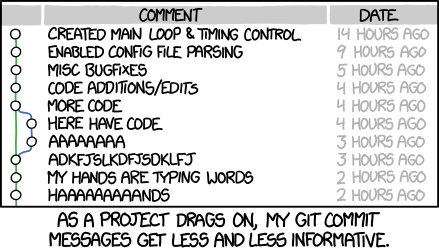
\includegraphics[scale=0.45]{xkcd_git_commit.png}
\caption{XKCD and Git Log\cite{website:xkcd_revision_history_comic}}
\end{figure}
\end{frame}

\begin{frame}
\frametitle{Writing Good Commit Messages}
\begin{enumerate}
\item{Separate subject from body with a blank line}
\item{Limit the subject line to 50 characters}
\item{Capitalize the subject line}
\item{Do not end the subject line with a period}
\item{Use the imperative voice in the subject line}
\item{Wrap the body at 72 characters}
\item{Use the body to explain what and why vs.\ how}
\end{enumerate}
\end{frame}

\begin{frame}[fragile]
\frametitle{Writing Good Commit Messages}
\framesubtitle{Why?}
Because \texttt{git-log} output \textit{needs} to be beautiful:
\lstinputlisting{code/gitlog}
\end{frame}

\begin{frame}[fragile]
  \frametitle{Writing Good Commit Messages}
  \framesubtitle{Examples}
\begin{Verbatim}[fontsize=\small]
i dont think this stuff is needed
\end{Verbatim}
\end{frame}

\begin{frame}[fragile]
  \frametitle{Writing Good Commit Messages}
  \framesubtitle{Examples}
\begin{Verbatim}[fontsize=\scriptsize]
Convert ROM read access enable/disable string parsing to use the
`kstrtobool` function.

This fixes Bugzilla Bug 111301 -- Sysfs PCI rom file functionality does
not match documentation.

bugzilla: https://bugzilla.kernel.org/show_bug.cgi?id=111301

Reported-by: googlegot@xxxxxxxxx
Signed-off-by: Kenny Ballou <kballou@xxxxxxxxxxxxxx>
\end{Verbatim}
\end{frame}

\begin{frame}[fragile]
  \frametitle{Writing Good Commit Messages}
  \framesubtitle{Examples}
\begin{Verbatim}[fontsize=\scriptsize]
object.h: update flag allocation comment

Since the "flags" is shared, it's a good idea to keep track of who
uses what bit. When we need to use more flags in library code, we can
be sure it won't be re-used for another purpose by some caller.

While at there, fix the location of "5" (should be in a different
column than "4" two lines down)

Signed-off-by: Nguyễn Thái Ngọc Duy <pclouds@gmail.com>
Signed-off-by: Junio C Hamano <gitster@pobox.com>
\end{Verbatim}
\end{frame}

\begin{frame}
  \frametitle{Writing Good Commit Messages}
  \begin{itemize}
    \item{Be consistent}
  \end{itemize}
\end{frame}

\subsection{git-pull}
\begin{frame}[fragile]
\frametitle{\texttt{git-pull} considered harmful}
\begin{itemize}
\item{Standard use of \texttt{git-pull} requires clean working directory}
\item{Will force a merge, if drift between remote and local}
\item{From the Git documentation~\cite{website:gitworkflows7}, ``Do not use
\texttt{git pull} unless you actually want to merge the remote branch.''}
\item{I personally prefer using \texttt{git-fetch} and \texttt{git-merge}}
\item{Another option: use \texttt{--ff-only} when pulling}
\end{itemize}
\lstinputlisting[title=\texttt{\~{}/.gitconfig}]{code/5/9}
\end{frame}

\subsection{Moving Forward}
\begin{frame}
\frametitle{Git± Moving Forward}
\begin{itemize}
\item<2->{Read the output}
\item<3->{No, \textit{really}, Read the output!}
\item<4->{\url{git-scm.com} and ``Pro Git''}
\item<5->{\texttt{\#{}git} on Freenode}
\item<6->{Git± man pages~\cite{website:git_man_pages}
~\cite{website:understand_git_man_pages}}
\item<7->{Git± workflows~\cite{website:gitworkflows7}}
\end{itemize}
\end{frame}

\section*{References}
\begin{frame}[allowframebreaks]
\frametitle{References}
\nocite{*}
\renewcommand{\refname}{}
\bibliographystyle{plain}
\bibliography{references}
\end{frame}

\againframe{titleslide}
\end{document}
